\documentclass[11pt,a4paper]{article}
\usepackage[T1]{fontenc}
\usepackage[utf8]{inputenc}
\usepackage[french]{babel}
\usepackage{lmodern}
\usepackage{geometry}
\usepackage{amsmath,amssymb}
\usepackage{booktabs}
\usepackage{graphicx}
\usepackage{hyperref}
\geometry{margin=2.4cm}

\title{Rapport formel round 3\\
\large Régimes dynamiques, observables finaux et carte de paramètres du modèle WIP}
\author{Codex}
\date{3 avril 2026}

\begin{document}
\maketitle

\begin{abstract}
Ce rapport remplace les corrections ponctuelles des versions precedentes par une formalisation plus compacte et plus predictive. L'objectif n'est plus seulement de commenter le code, mais de construire un modele formel suffisant pour comprendre et regler les observables finaux du WIP: densite du reseau de credit, flux de transactions, faillites par pas, propagation secondaire et survie de population. Trois resultats ressortent. Premierement, le WIP doit etre decrit comme un systeme discret dirige par deux secteurs distincts: un secteur de \emph{flux} (transactions, faillites, propagation) qui atteint un quasi-regime apres un temps d'installation, et un secteur de \emph{stocks} (nombre de prets actifs, fragilite cachee) qui continue de deriver a cause de $\tau=0$. Deuxiemement, le bon substitut empirique au ``proxy spectral'' precedent n'est pas une fraction globale de faillites contaminees, mais deux observables distinctes: la part des faillites qui etaient solvables avant la resolution et le nombre de faillites secondaires par faillite deja fragile. Troisiemement, la carte de parametres montre que $k$ controle la topologie, $\theta$ le levier, et $\lambda$ le renouvellement de population. Pour construire un reseau dense avec avalanches persistantes, le regime le plus propre est obtenu autour de $k=3$, $\theta \in [0.35,0.5]$ et $\lambda \approx 2$; un regime plus agressif de type ``feu de foret'' est atteint vers $k=3$, $\theta \approx 0.7$, $\lambda \approx 2$.
\end{abstract}

\section{Objet du rapport}
Les deux critiques de second tour imposent quatre corrections de fond:
\begin{itemize}
\item distinguer les corrections exactes du code et les fermetures de champ moyen;
\item cesser de melanger un critere spectral theorique avec un indicateur empirique mal defini;
\item dater explicitement le passage du transitoire au quasi-regime;
\item fournir une carte de parametres utilisable pour viser un reseau dense avec avalanches.
\end{itemize}

Le present rapport complete donc les papiers precedents au lieu de les prolonger ligne par ligne. Il s'appuie sur:
\begin{itemize}
\item un batch long par defaut sur $4$ seeds et $1000$ pas;
\item un sweep en $k$ a $\theta=0.35$, $\lambda=2$;
\item une carte $(\theta,\lambda)$ a $k=3$;
\item des figures de dynamique temporelle et de regime.
\end{itemize}

\section{Noyau formel corrige}
\subsection{Identites discretes minimales}
On note:
\[
N_t = \text{nombre d'entites vivantes},\qquad
M_t = \text{nombre de prets actifs},\qquad
\ell_t = \frac{1}{N_t}\sum_i L_i(t),\qquad
p_t = \frac{1}{N_t}\sum_i P_i(t).
\]
Le WIP se lit au premier ordre comme l'application discrete:
\[
X_{t+1} = \mathcal F(X_t),
\]
avec decomposition
\[
\mathcal F=
\mathcal U \circ
\mathcal F_{\mathrm{fail}} \circ
\mathcal C \circ
\mathcal D \circ
\mathcal A \circ
\mathcal I \circ
\mathcal E \circ
\mathcal S \circ
\mathcal B.
\]

Les identites de population et de graphe sont:
\[
N_{t+1}-N_t = \Xi_t - F_t,
\qquad
M_{t+1}-M_t = T_t - E_t,
\]
ou $\Xi_t$ est le nombre de naissances, $F_t$ le nombre de faillites resolues, $T_t$ le nombre de nouveaux prets, et $E_t$ le nombre effectif d'extinctions de prets par revalorisation, amortissement ou faillite.

Pour les grandeurs liquides et productives, une decomposition utile est:
\[
\ell_{t+1}-\ell_t
=
\Pi^{\mathrm{eff}}_t
-D^\ell_t
-X_t
\;+\;
\varepsilon^\ell_t,
\]
\[
p_{t+1}-p_t
=
X_t
+Y_t
-D^p_t
-\Psi_t.
\]
Ici:
\begin{itemize}
\item $\Pi^{\mathrm{eff}}_t=\frac{1}{N_t}\sum_i \alpha_i(t)\sqrt{P_i(t)}$;
\item $D^\ell_t$ est la depreciation liquide moyenne;
\item $X_t$ est l'auto-investissement moyen;
\item $Y_t$ est l'injection moyenne de taille productive par nouveaux prets;
\item $\Psi_t$ est la destruction de taille par faillites;
\item $\varepsilon^\ell_t$ regroupe les flux liquides nets dus a l'activite de credit, aux cessions et aux write-downs.
\end{itemize}

Cette ecriture remplace avantageusement l'ancien terme ferme $+\iota m_t$. Le signe et la taille de $\varepsilon^\ell_t$ sont des objets empiriques de second ordre; ils ne doivent pas etre hypostases en terme principal sans calibration.

\subsection{Correction de richesse nette}
La correction fondamentale deja identifiee reste:
\[
\Delta NW_i^{\mathrm{endo}} = -x_i.
\]
L'auto-investissement diminue donc la richesse nette bilancielle \emph{au moment de l'operation}. Il ne faut pas le decrire comme un simple effet de flux futur. En revanche, l'effet instantane du pret au deblocage est nul sur la richesse nette \emph{si} les postes miroirs du pret se compensent a l'instant du deblocage; c'est un mecanisme distinct, et il ne doit plus etre confondu avec l'auto-investissement.

\subsection{Fragilite cachee}
La fragilite cachee est definie exactement par
\[
H_t = \sum_{e \in \mathcal L_t} q_e(t)\Big(1-(1-\delta_{\mathrm{exo}})^{a_e(t)}\Big).
\]
Pour un pret survivant d'age $a$,
\[
\Delta H_e
=
q_e\,\delta_{\mathrm{exo}}(1-\delta_{\mathrm{exo}})^a.
\]
D'ou, au niveau agrégé,
\[
H_{t+1}-H_t
\approx
\delta_{\mathrm{exo}}
\sum_{e \in \mathcal L_t}
q_e(t)(1-\delta_{\mathrm{exo}})^{a_e(t)}
\;-\;
\Omega_t,
\]
ou $\Omega_t$ regroupe les effacements par revalorisation, amortissement et faillite.

La fermeture grossiere
\[
\delta_{\mathrm{exo}}\,M_t\bar q_t
\]
n'est recevable que si le portefeuille est jeune, c'est-a-dire si
\[
\delta_{\mathrm{exo}}\bar a_t \ll 1.
\]
Quand $\tau=0$ et que les prets s'accumulent, cette hypothese n'est plus automatique. La bonne fermeture doit donc conserver un facteur d'age moyen, ou renoncer a fermer completement $H_t$.

\subsection{Deux metriques de propagation, pas un pseudo-rayon spectral}
Le critere spectral theorique $\rho(\mathcal B_t)$ reste un objet de linearisation. Il n'est pas estime ici. A sa place, nous utilisons deux metriques empiriques distinctes.

Pour une cascade au pas $t$:
\begin{itemize}
\item $F_t$ = nombre total de faillites du pas;
\item $C_t$ = nombre de faillites qui etaient solvables avant la resolution;
\item $G_t$ = nombre de faillites deja fragiles au debut de la resolution.
\end{itemize}
On definit alors:
\[
s_t^{\mathrm{sec}} = \frac{C_t}{F_t},
\qquad
R_t^{\mathrm{sec}} = \frac{C_t}{G_t}.
\]

$s_t^{\mathrm{sec}}$ mesure la \emph{part secondaire} d'un episode. $R_t^{\mathrm{sec}}$ mesure les \emph{faillites secondaires par faillite primaire fragile}. Aucune de ces deux quantites n'est un rayon spectral. En revanche, $R_t^{\mathrm{sec}}$ est un proxy branching beaucoup plus proche de l'idee de reproduction locale que l'ancien ratio global.

\section{Diagnostic de regime du scenario de reference}
\subsection{Flux quasi-stationnaires, stocks derivants}
La critique de non-stationnarite etait juste. La figure~\ref{fig:ref-time} montre une rupture nette avant/apres $t \approx 500$.

\begin{figure}[t]
\centering
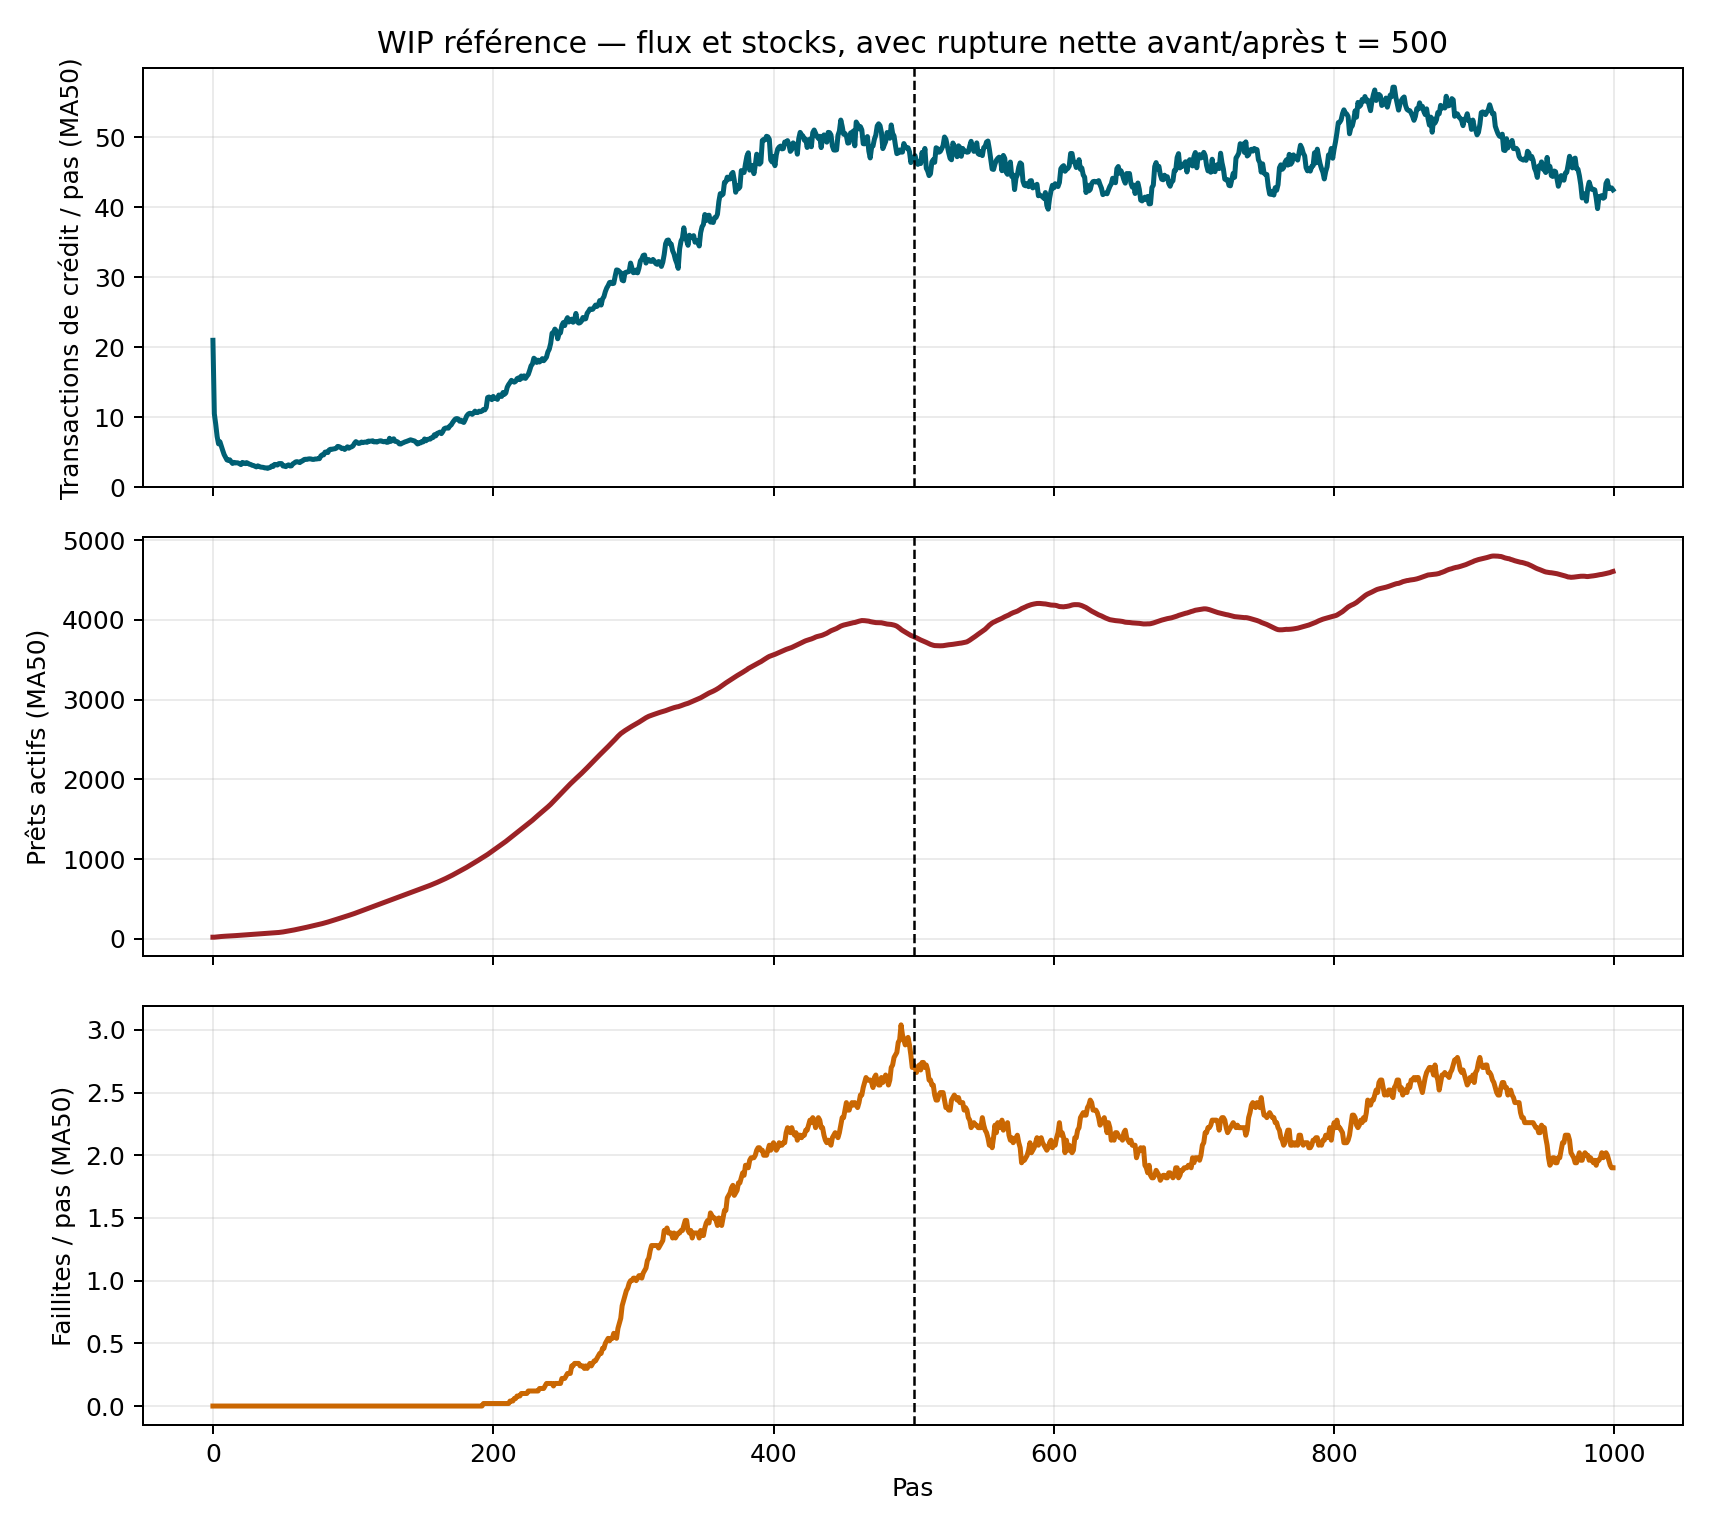
\includegraphics[width=0.96\textwidth]{../data/round3/figures/reference_timeseries.png}
\caption{Scenario de reference du WIP. Les flux de transactions et de faillites entrent dans un quasi-regime apres environ $500$ pas. Le stock de prets actifs, lui, continue de croitre lentement parce que $\tau=0$.}
\label{fig:ref-time}
\end{figure}

Les fenetres temporelles confirment cette lecture:
\begin{center}
\small
\begin{tabular}{lrrrr}
\toprule
Fenetre & tx/pas & prets actifs & faillites/pas & second./fragiles \\
\midrule
$0$--$500$   & $26.51$ & $2092.52$ & $0.968$ & $0.163$ \\
$500$--$1000$ & $47.04$ & $4255.40$ & $2.228$ & $0.491$ \\
\bottomrule
\end{tabular}
\end{center}

Les pentes sur $500$--$1000$ montrent en outre une asymetrie structurelle:
\begin{itemize}
\item transactions et faillites: pente relative par pas $\approx 7.7\times 10^{-5}$, donc quasi-plateau de flux;
\item prets actifs: pente relative par pas $\approx 4.2\times 10^{-4}$, donc derive de stock encore visible.
\end{itemize}

La bonne conclusion n'est donc pas ``le systeme est stationnaire'', mais:
\begin{quote}
le WIP presente un quasi-regime des \emph{flux} apres installation, tandis que les \emph{stocks} continuent de deriver tant que l'amortissement reste nul et que la revalorisation n'est pas globale.
\end{quote}

\subsection{Survie: la cohorte suivie n'est pas la population}
Le code suit:
\begin{itemize}
\item toutes les entites initiales;
\item environ $3\%$ des entites creees apres $t=0$.
\end{itemize}
La cohorte ``162 entites suivies'' des versions precedentes n'etait donc pas un echantillon representatif uniforme.

Dans la nouvelle etude, la survie est calculee directement sur la population complete des entites simulees. Sur $4$ seeds, $1000$ pas, on obtient:
\begin{itemize}
\item population complete: $\mathrm{RMST}_{1000}\approx 334.5 \pm 15.2$ et $S(1000)\approx 0.0865 \pm 0.0063$;
\item cohorte initiale: $\mathrm{RMST}_{1000}\approx 606.1 \pm 35.5$;
\item entites nees apres $t=0$: $\mathrm{RMST}_{1000}\approx 317.7 \pm 14.4$.
\end{itemize}
L'ecart entre cohorte initiale et cohortes nees en regime dense suffit a montrer que la survie de la cohorte suivie ne doit plus etre utilisee comme estimateur principal.

\subsection{Regime tardif du scenario par defaut}
Sur le batch long par defaut ($k=3$, $\theta=0.35$, $\lambda=2$), fenetre $500$--$1000$, on mesure:
\begin{itemize}
\item transactions de credit: $45.50 \pm 0.95$ par pas;
\item prets actifs: $4265.9 \pm 33.5$;
\item prets actifs par entite: $6.93 \pm 0.29$;
\item faillites: $2.189 \pm 0.036$ par pas;
\item part secondaire: $0.305 \pm 0.015$;
\item secondaires par fragile: $0.439 \pm 0.031$;
\item ratio final de fragilite cachee: $0.894 \pm 0.012$.
\end{itemize}

Le dernier chiffre est important: en regime tardif, la valeur nominale des creances surestime fortement leur valeur economique. Le WIP n'est donc pas seulement dense; il est dense et latentement sur-evalue.

\section{Carte de parametres}
\subsection{Le seuil topologique est porte par $k$}
La figure~\ref{fig:k-sweep} montre un saut clair entre $k=2$ et $k=3$.

\begin{figure}[t]
\centering
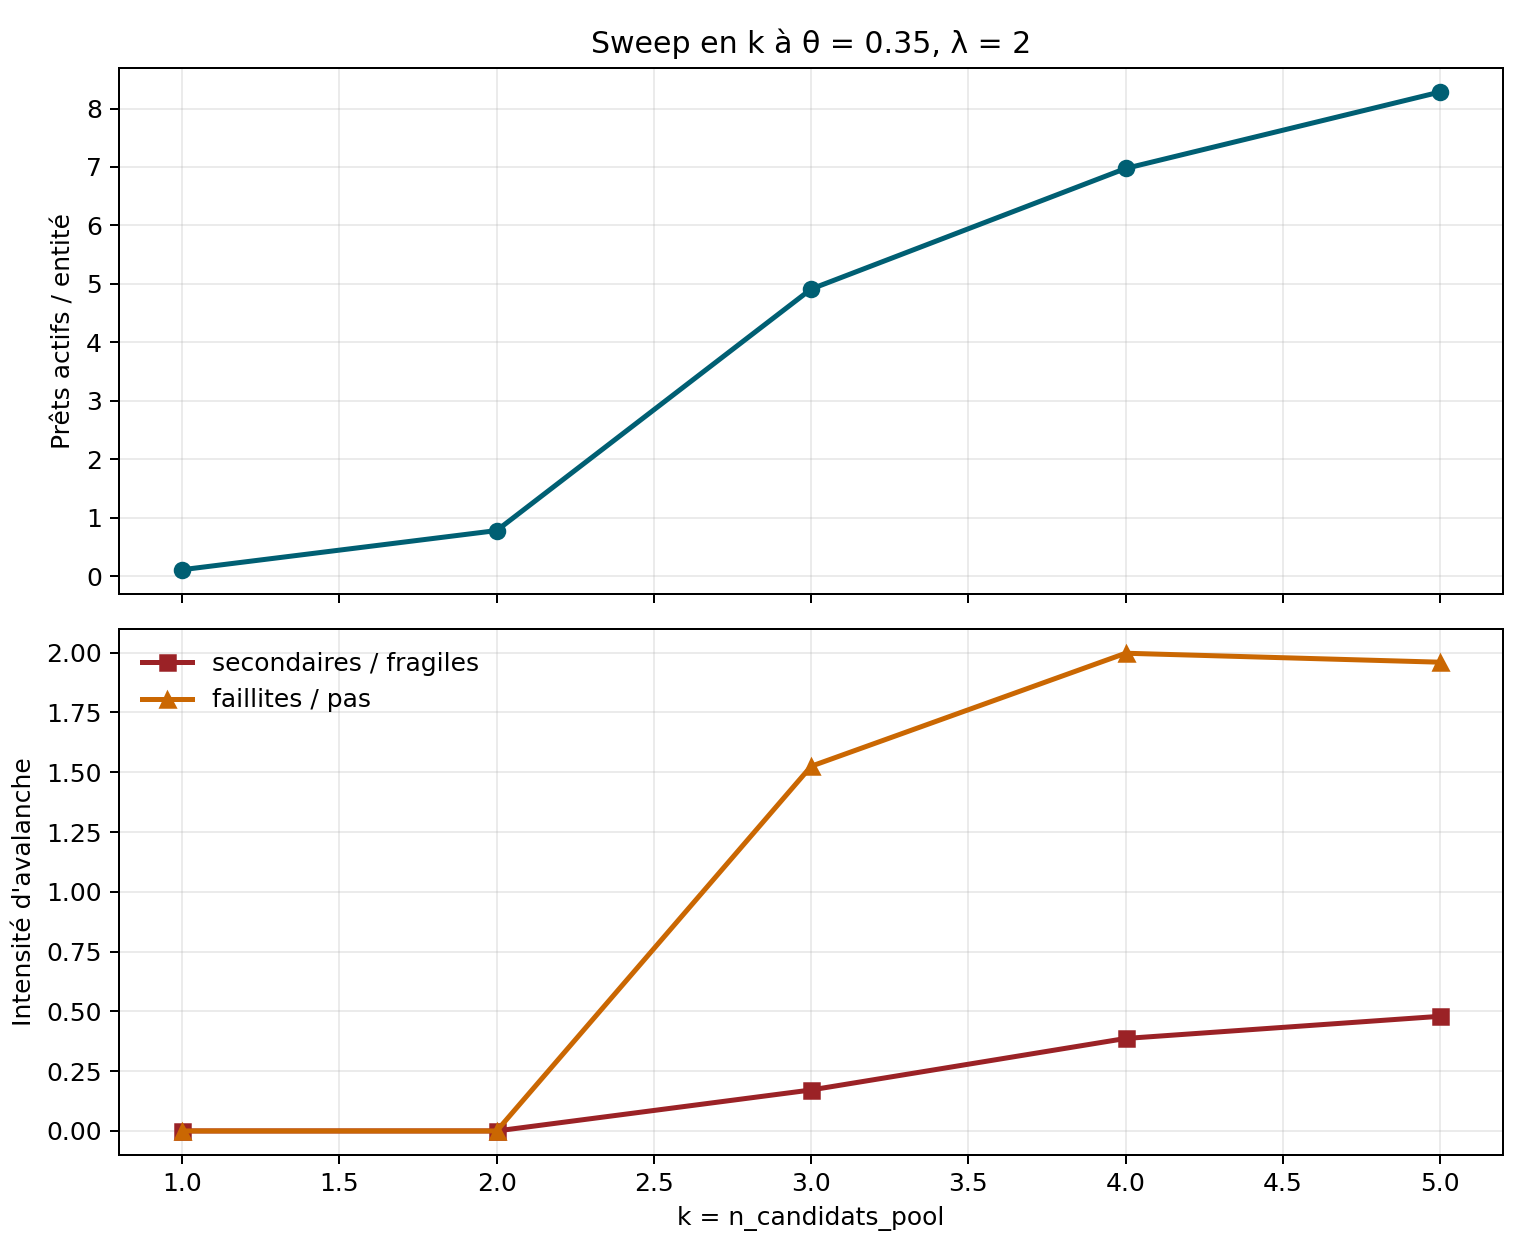
\includegraphics[width=0.85\textwidth]{../data/round3/figures/k_sweep_summary.png}
\caption{Sweep en $k$ a $\theta=0.35$, $\lambda=2$. Pour $k\le 2$, pas d'avalanche. A partir de $k=3$, densite et propagation deviennent positives; $k\ge 4$ renforce encore la propagation mais au prix d'une destruction de population plus forte.}
\label{fig:k-sweep}
\end{figure}

Les moyennes tardives sur $400$ pas sont:
\begin{center}
\small
\begin{tabular}{rrrr}
\toprule
$k$ & prets/entite & faillites/pas & second./fragiles \\
\midrule
$1$ & $0.11$ & $0.00$ & $0.00$ \\
$2$ & $0.78$ & $0.00$ & $0.00$ \\
$3$ & $4.91$ & $1.53$ & $0.17$ \\
$4$ & $6.98$ & $2.00$ & $0.39$ \\
$5$ & $8.28$ & $1.96$ & $0.48$ \\
\bottomrule
\end{tabular}
\end{center}

Interpretation: $k$ est le parametre de \emph{percolation topologique}. Tant que $k\le 2$, le reseau reste trop segrege pour former une intermediation endogene contagieuse. $k=3$ est le premier regime dense et contagieux. $k\ge 4$ densifie encore, mais l'attrition devient plus couteuse.

\subsection{La carte $(\theta,\lambda)$ a $k=3$}
Les deux figures suivantes resument le compromis principal.

\begin{figure}[t]
\centering
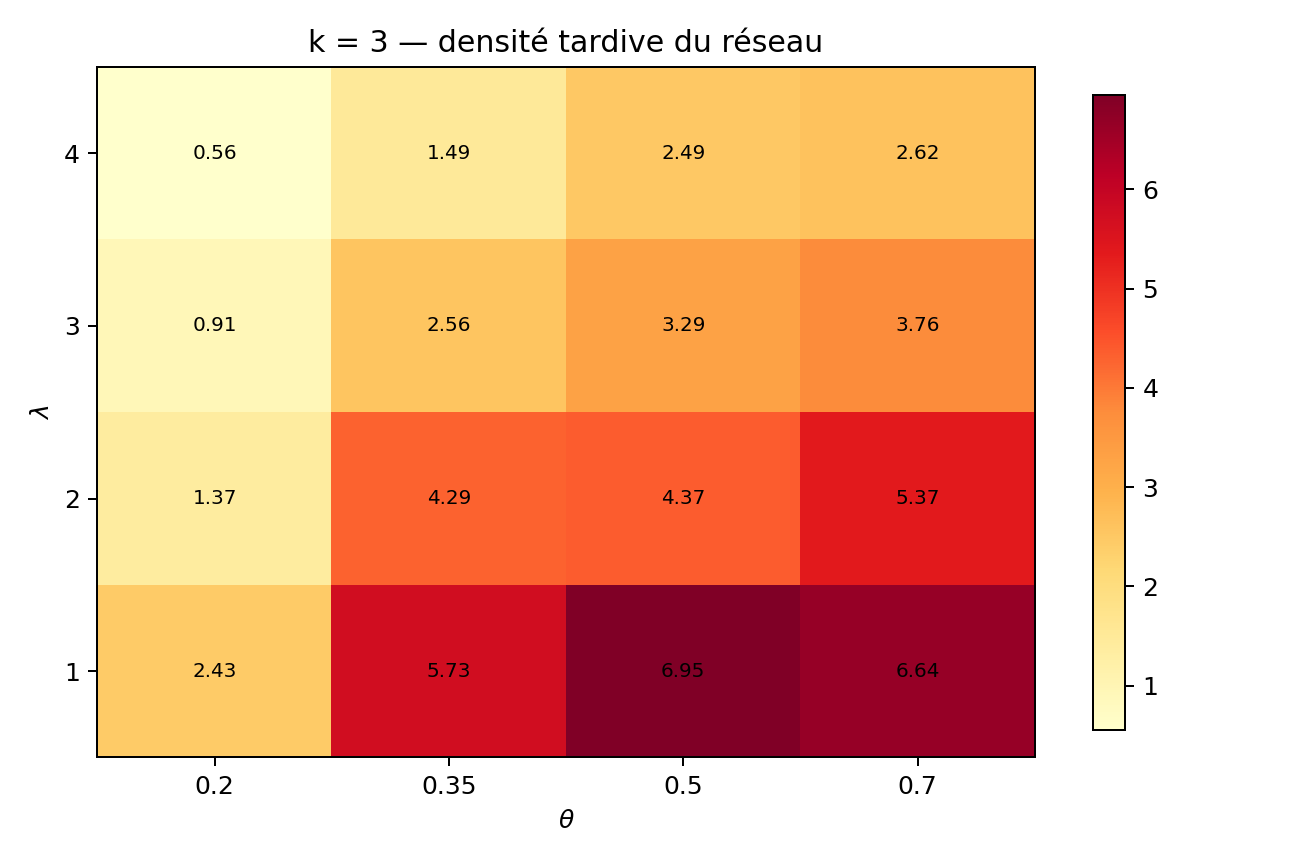
\includegraphics[width=0.47\textwidth]{../data/round3/figures/theta_lambda_density_k3.png}
\hfill
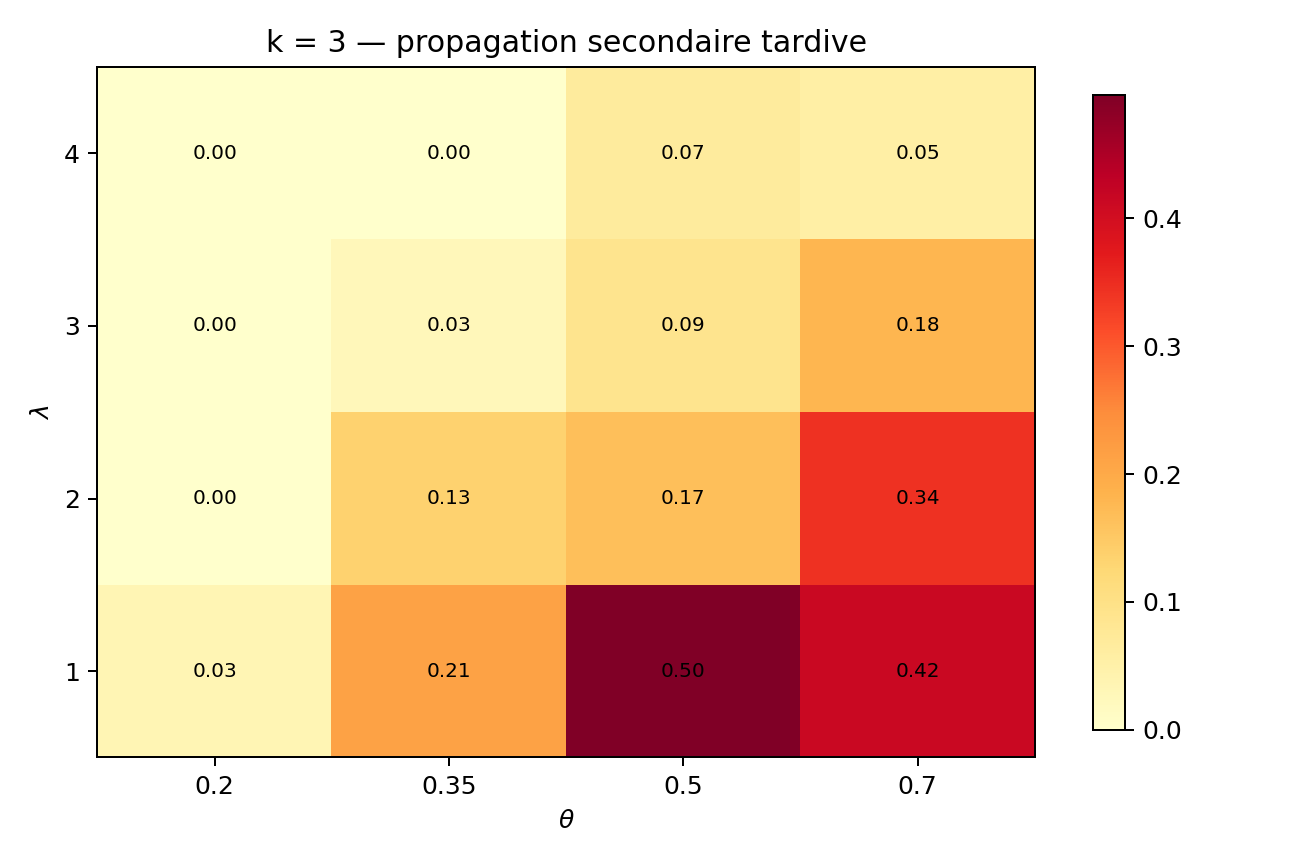
\includegraphics[width=0.47\textwidth]{../data/round3/figures/theta_lambda_secondary_k3.png}
\caption{Carte de regime a $k=3$. Gauche: densite tardive du reseau. Droite: propagation secondaire tardive.}
\label{fig:theta-lambda}
\end{figure}

La lecture mecanique est simple:
\begin{itemize}
\item $\theta$ controle le levier. Quand $\theta$ augmente, le volume de credit et la propagation secondaire montent presque monotoniquement;
\item $\lambda$ controle le renouvellement. Trop faible, le systeme devient petit et tres destructif; trop grand, il se remplit d'entites jeunes et liquides, ce qui dilue la contagion.
\end{itemize}

Le bon analogon du ``feu de foret'' est donc:
\begin{quote}
\textbf{connectivite suffisante} ($k\ge 3$) + \textbf{levier intermediaire a fort} ($\theta$) + \textbf{renouvellement intermediaire} ($\lambda$).
\end{quote}

\subsection{Regimes recommandes}
On peut distinguer trois usages.

\paragraph{Regime de compromis dense avec avalanches soutenues.}
\[
k=3,\qquad \theta \in [0.35,0.5],\qquad \lambda \approx 2.
\]
On obtient alors environ $4.3$ prets actifs par entite, $1.16$ a $1.31$ faillites par pas, et $0.135$ a $0.166$ faillite secondaire par faillite fragile initiale. La population finale reste entre environ $630$ et $670$ entites sur l'horizon de comparaison.

\paragraph{Regime agressif de type ``feu de foret''.}
\[
k=3,\qquad \theta \approx 0.7,\qquad \lambda \approx 2.
\]
La densite monte a environ $5.37$ prets par entite et la propagation secondaire a environ $0.344$, au prix d'une population finale plus basse ($\approx 530$).

\paragraph{Regime a propagation maximale mais population reduite.}
\[
k=3,\qquad \lambda = 1,\qquad \theta \in [0.5,0.7].
\]
La densite et la propagation sont maximales dans notre carte ($6.64$ a $6.95$ prets par entite; $0.42$ a $0.50$ secondaires par fragile), mais la population moyenne tombe vers $240$--$254$ entites. C'est un regime de criticite forte, pas un regime durable.

\section{Consequences pour la modelisation predictive}
La reduction precedente permet de predire qualitativement les observables finaux:
\begin{itemize}
\item si $k\le 2$, alors le graphe reste trop mince: faible densite, pas de propagation;
\item si $k\ge 3$ mais $\theta$ est trop faible, le reseau se densifie peu et les avalanches restent nulles ou faibles;
\item si $k\ge 3$ et $\theta$ augmente, le reseau se densifie et la propagation monte;
\item si $\lambda$ devient trop grand, la population rajeunit plus vite que le reseau ne vieillit: la densite et la propagation baissent;
\item si $\lambda$ est trop faible, on garde des portefeuilles ages et fragiles, mais sur une population faible.
\end{itemize}

Autrement dit, le WIP ne doit pas etre pilote par un seul ``parametre critique''. Il faut au moins trois axes:
\begin{enumerate}
\item un axe topologique ($k$);
\item un axe de levier ($\theta$);
\item un axe de renouvellement ($\lambda$).
\end{enumerate}

La bonne variable de sortie n'est pas seulement le nombre brut de faillites, mais le triplet:
\[
\big(m^{\mathrm{late}},\, f^{\mathrm{late}},\, R_{\mathrm{sec}}^{\mathrm{late}}\big)
=
\left(
\overline{\frac{M_t}{N_t}},
\overline{F_t},
\frac{\sum C_t}{\sum G_t}
\right)_{\mathrm{fenetre\ tardive}}.
\]
Ce triplet resume respectivement la densite du reseau, le debit de destruction, et la part proprement propagative des cascades.

\section{Remarques sur le parametre d'amortissement}
Un test cible hors sweep principal montre qu'une petite amortisation change le regime de facon non monotone. A $500$ pas, $\tau=0.01$ peut presque annuler la derive locale du stock de prets tout en conservant des faillites et de la propagation. En revanche, sur $1000$ pas et seed $42$, la derive du stock redevient positive. Il serait donc premature d'affirmer qu'un petit $\tau>0$ ``resout'' la non-stationnarite. En pratique:
\begin{itemize}
\item $\tau$ est bien un levier de regulation des stocks;
\item mais il interagit fortement avec le debit de nouvelles transactions;
\item une vraie stationnarite des stocks requerra probablement soit un amortissement plus structurel, soit une revalorisation plus frequente des creances.
\end{itemize}

\section{Errata minimaux sur v2}
Le modele \texttt{v2} reste utile comme base de comparaison, mais il faut corriger sa lecture formelle sur six points:
\begin{itemize}
\item l'auto-investissement y reduit aussi la richesse nette instantanee;
\item la quantite diagnostique de derive doit employer $\bar \Pi(p)$ et non $\alpha\sqrt p$ comme identite exacte;
\item les resultats a $300$ pas et a $1000$ pas ne sont pas directement comparables, car les stocks y accumulent encore;
\item la fermeture du hazard reste ouverte;
\item la condition d'acceptation du credit reste seulement partiellement fermee;
\item la difference entre $q_{\max}$ de \texttt{v2} et de \texttt{v3/WIP} vient du fait que \texttt{v3/WIP} soustrait explicitement le surplus deja mobilisable $S_b$, alors que \texttt{v2} ne le fait pas.
\end{itemize}
Ces points sont mineurs pour la logique du present rapport, car la carte de regimes dense-avalanches est une propriete du WIP, pas de \texttt{v2}.

\section{Conclusion}
Le resultat principal de cette passe est conceptuellement simple. Le WIP n'est pas encore un modele stationnaire complet de type SOC canonique; c'est un systeme discret dirige, a flux quasi-stationnaires mais a stocks encore derivants, dans lequel la criticite depend d'un compromis entre topologie, levier et renouvellement.

La bonne facon de le regler pour obtenir un reseau dense avec avalanches n'est donc pas ``augmenter le hasard'' ou ``augmenter la creation'', mais:
\begin{itemize}
\item franchir le seuil topologique $k=3$;
\item choisir un levier $\theta$ suffisant pour charger le reseau;
\item maintenir $\lambda$ dans une zone intermediaire ou la population ne soit ni trop rare, ni trop juvenile.
\end{itemize}

Pour un usage exploratoire robuste, nous recommandons:
\[
k=3,\qquad \theta \in [0.35,0.5],\qquad \lambda \approx 2.
\]
Pour un regime plus incendiaire et plus proche de l'image ``foret auto-critique'', on peut pousser vers
\[
k=3,\qquad \theta \approx 0.7,\qquad \lambda \approx 2,
\]
en acceptant une destruction de population plus forte.

\end{document}
